\newpage


\section{Wyniki testów i analiza}\label{sec:testy}

Przeprowadzono serię testów manualnych mających na celu weryfikację poprawności działania scrapera i sklepu internetowego z uwzględnieniem wdrożonych metod detekcji web scrapingu.
Testy obejmowały 5 różnych scenariuszy tj.:
\begin{enumerate}[label={scenariusz \arabic*:},labelindent=\parindent, leftmargin=*]
    \item bez zabezpieczeń,
    \item tylko Bot Blocker Reverse Proxy,
    \item tylko rate limiting,
    \item tylko zabezpieczenie wykorzystujące browser fingerprinting,
    \item włączone wszystkie zabezpieczenia.
\end{enumerate}

\subsection{Scenariusz 1: Bez Zabezpieczeń}\label{subsec:scenariusz-1:-wyaczone-zabezpieczenia}

Scenariusz 1 stanowi punkt odniesienia dla dalszych testów.
Testy te przeprowadzono dwukrotnie:
przez wdrożeniem metod opisanych w \autoref{sec:wdrozenie-metod-detekcji}
oraz po ich wdrożeniu i wyłączeniu.

Zarówno scaper, jak też sklep internetowy działały zgodnie z oczekiwaniami.
Scraper nie został zablokowany i pobrał szczegółowe dane o wszystkich produktach w sklepie.
Sklep spełniał wszystkie wymogi funkcjonalne.
Użytkownik miał możliwość swobodnego przeglądania asortymentu i dokonywania procesu zakupowego.
Korzystanie z serwisu przekładało się na płynne i komfortowe doświadczenia zakupowe.

\subsection{Scenariusz 2: Włączone zabezpieczenie Bot Blocker Reverse Proxy}\label{subsec:scenariusz-3:-waczone-zabezpieczenie-reverse-proxy-bot-blocker}

Scenariusz 2 zakłada włączenie metody detekcji web scrapingu opisywanej w \autoref{subsec:reverse-proxy-impl}.
Przetestowano scraper i aplikacje sklepu internetowego wraz z zabezpieczeniem Bot Blocker Reverse Proxy.

Funkcjonowanie sklepu internetowego z perspektywy użytkownika końcowego nie uległo zmianie względem scenariusza 1.

Wykonano szereg poleceń \texttt{curl}, z czego każde posiadało nagłówek \texttt{User-Agent} lub \texttt{Referer} z wartością zawartą na czarnej liście (ang. \emph{blacklist}).
Część wykonanych poleceń została przedstawiona na \autoref{lst:bot-blocker-proxy}.
Żądania zawierające takie nagłówki otrzymały odpowiedź \texttt{error code: 502}, podczas gdy inne działały bez zmian.

Uruchomiono scraper i nie zaobserwowano żadnych różnic względem scenariusza 1.
Wynika to z faktu, że podczas implementacji scrapera zostały ustawione nagłówki, które są standardowo wysyłane przez użytkownika sklepu (zob. \autoref{subsubsec:storeclient}).

\begin{listing}[H]
    \begin{minted}[xleftmargin=10pt,linenos,breaklines]{bash}
$ curl 'https://api.tulski.com/store/products?limit=1' --user-agent "404checker.com"
error code: 502
$ curl 'https://api.tulski.com/store/products?limit=1' --user-agent "AiBot"
error code: 502
$ curl 'https://api.tulski.com/store/products?limit=1' --referer "https://footbalive.org/"
error code: 502
$ curl 'https://api.tulski.com/store/products?limit=1' --referer "https://footbalive.org/"
error code: 502
$ curl 'https://api.tulski.com/store/products?limit=1' --referer "http://zx6.ru"
error code: 502
    \end{minted}
    \caption{Polecenia testujące Bot Blocker Reverse Proxy}
    \label{lst:bot-blocker-proxy}
\end{listing}

Testy potwierdzają poprawność implementacji, jednocześnie uwydatniając jej słabe strony.
Filtrowanie oparte na czarnej liście (ang. \emph{blacklist}) sprawdzi się w przeciwdziałaniu aktywności powszechnie znanych i nieskomplikowanych botów.

\subsection{Scenariusz 3: Włączony Rate Limiting}\label{subsec:scenariusz-2:-waczony-rate-limiting}

Scenariusz 3 obejmuje testy scrapera i sklepu internetowego z zabezpieczeniem opisywanym w \autoref{subsec:rate-limiting-impl}.

Testy rozpoczęto od weryfikacji obecności i poprawności implementacji mechanizmu rate limitingu.
Wykorzystano prosty skrypt \texttt{bash} (zob. \autoref{lst:bash-rate-limit}).
Po uruchomieniu skryptu zaobserwowano odpowiedzi z kodem 429, co potwierdza obecność polityki ograniczającej częstotliwość zapytań.
Dodatkowo, równocześnie z działaniem wyżej wymienionego skryptu, przeprowadzono testy komunikacji ze Store API z innego adresu IP\@  --- te nie zostały zablokowane.

\begin{listing}[H]
    \begin{minted}[xleftmargin=10pt,linenos,breaklines]{bash}
#!/bin/bash

while :;
do
  curl -X GET 'https://api.tulski.com/store/products?limit=1' \
        -s \
        -o /dev/null \
        -w "$(date "+%H:%M:%S") GET /store/products?limit=1 %{http_code}\n" &
  sleep 0.2
done
    \end{minted}
    \caption{Skrypt bash weryfikujący obecność zabezpieczenia rate limiting}
    \label{lst:bash-rate-limit}
\end{listing}

Stwierdzono, że polityka ograniczająca częstotliwość zapytań (\emph{rate limit}) nie wpływa na doświadczenia użytkowników końcowych sklepu tulski.
Reguły skonfigurowano prawidłowo.
Wszystkie widoki i elementy ładują się zgodnie z oczekiwaniami.

W dalszej części testów skupiono się na działaniu scrapera.
Po jego uruchomieniu w logach zauważono odpowiedzi z kodem 429 (zob. \autoref{lst:rate-limiting-scraper-logs}).
Scraperowi udało się pobrać szczegółowe dane dla jedynie 28 produktów.
Po 3 zablokowanych żądaniach o szczegóły dla jednego z produktów proces zakończył się błędem ~\mintinline{text}{HTTPError}.
Zabezpieczenie skutecznie zablokowało aktywność scrapera.

Należy jednak nadmienić, że web scraping sklepu tulski jest nadal teoretycznie możliwy.
Wymagałoby to zmodyfikowania obecnego scrapera, tak aby spowolnił tempo wysyłania żądań i/lub wykorzystywał proxy.

\begin{listing}[p]
    \begin{minted}[xleftmargin=10pt,linenos,breaklines,fontsize=\scriptsize]{text}
10:50:23.112 debug: GET /store/products&is_giftcard=false&limit=500 200 OK
10:50:23.308 debug: GET /store/products/prod_01HDFP2JMEF8AHJA47GHZN5TH7 429 Too Many Requests
10:50:23.310 debug: GET /store/products/prod_01HDFP2NPH1J7129PEE65XJ5MX 429 Too Many Requests
10:50:23.312 debug: GET /store/products/prod_01HDFP2MT60JEYPKS5YDZEYF2H 429 Too Many Requests
10:50:23.312 debug: GET /store/products/prod_01HDFP2KXGNN6JDVGB5ZFF1DQP 429 Too Many Requests
10:50:23.313 debug: GET /store/products/prod_01HDFP2HJ2DGQFJQ61SP7X2K11 429 Too Many Requests
10:50:23.314 debug: GET /store/products/prod_01HDFP2KXP93SBT1RTG6XM8W4G 429 Too Many Requests
10:50:23.314 debug: GET /store/products/prod_01HDFP2JW0QSF2594GASXW4MPF 429 Too Many Requests
10:50:23.315 debug: GET /store/products/prod_01HDFP2KXVD6Z1SB9JV8HY2GE7 429 Too Many Requests
10:50:23.316 debug: GET /store/products/prod_01HDFP2M0ETB579GN2EHN3B83A 429 Too Many Requests
10:50:23.317 debug: GET /store/products/prod_01HDFP2M00BHH070Z02B1G3Z8H 429 Too Many Requests
10:50:23.318 debug: GET /store/products/prod_01HDFP2PJHJHZ6N1S2W0E3RXP9 429 Too Many Requests
10:50:23.318 debug: GET /store/products/prod_01HDFP2NQDG1MJSDCWWMZNJ7XW 429 Too Many Requests
10:50:23.319 debug: GET /store/products/prod_01HDFP2JJKJBE17TK77WZMRGYE 429 Too Many Requests
10:50:23.319 debug: GET /store/products/prod_01HDFP2M08GF76G15PD412AF4R 429 Too Many Requests
10:50:23.320 debug: GET /store/products/prod_01HDFP2MT8T6G3ABK70KFVYEBP 429 Too Many Requests
10:50:23.321 debug: GET /store/products/prod_01HDFP2HC05F595MXF5FJ64X1Y 429 Too Many Requests
10:50:23.321 debug: GET /store/products/prod_01HDFP2JSD0AVKRNGJVJ7P2YDD 429 Too Many Requests
10:50:23.321 debug: GET /store/products/prod_01HDFP2MSD9BGNVE6END09QWVR 429 Too Many Requests
10:50:23.322 debug: GET /store/products/prod_01HDFP2JN39STBMGJ8EG5X5HSA 429 Too Many Requests
10:50:23.322 debug: GET /store/products/prod_01HDFP2HEC6TD86HD25Z6ARK5T 429 Too Many Requests
10:50:23.323 debug: GET /store/products/prod_01HDFP2HHFVKWCGSKP8T5KCWW3 429 Too Many Requests
10:50:23.323 debug: GET /store/products/prod_01HDFP0FH8B6T1NY7E2ZF86WKV 429 Too Many Requests
10:50:23.324 debug: GET /store/products/prod_01HDFP0ESEJ9DKVD0YMBF7FSCB 429 Too Many Requests
10:50:23.324 debug: GET /store/products/prod_01HDFP2NNFZN5MFGHPEKKX5Z2T 429 Too Many Requests
10:50:23.325 debug: GET /store/products/prod_01HDFP0EMHR9PZV07YM5VWZSY7 429 Too Many Requests
10:50:23.325 debug: GET /store/products/prod_01HDFP0EP1JZJTPMWDWNS2EX7S 429 Too Many Requests
10:50:23.326 debug: GET /store/products/prod_01HDFP2KXQ6XX0AB5AZJ9WMJCM 429 Too Many Requests
10:50:23.326 debug: GET /store/products/prod_01HDFP2GRFQ9JQ45WTG04GSSA4 429 Too Many Requests
10:50:23.327 debug: GET /store/products/prod_01HDFP2HEYKC6YHAJ49GYYW35V 429 Too Many Requests
10:50:23.327 debug: GET /store/products/prod_01HDFP2JMFE8S0JTFK062VH3QJ 429 Too Many Requests
10:50:23.327 debug: GET /store/products/prod_01HDFP0EM88B18A7CE61K1MP3N 429 Too Many Requests
10:50:23.328 debug: GET /store/products/prod_01HDFP2JM7WE94EJBHF8HZERX2 429 Too Many Requests
10:50:23.328 debug: GET /store/products/prod_01HDFP0EMG75JVGRBCAPVFNC9C 429 Too Many Requests
10:50:23.329 debug: GET /store/products/prod_01HDFP0DP3TW570JRYF4EJJQ8N 429 Too Many Requests
10:50:23.329 debug: GET /store/products/prod_01HDFP0DNVF9PM11K0Y9VGAG96 429 Too Many Requests
10:50:23.330 debug: GET /store/products/prod_01HDFP0FCDW9Q3DBAGHR3KSWQT 429 Too Many Requests
10:50:23.330 debug: GET /store/products/prod_01HDFP0G9HD2J7T9TVK5C76QGB 429 Too Many Requests
10:50:23.331 debug: GET /store/products/prod_01HDFP0CAJ3XYBBXW4DXSJYFN0 429 Too Many Requests
10:50:23.331 debug: GET /store/products/prod_01HDFP2JX7ET99T5J368NV8NQF 429 Too Many Requests
10:50:23.331 debug: GET /store/products/prod_01HDFP2HGY5MHZXZRJS5SY1NEX 429 Too Many Requests
10:50:23.331 debug: GET /store/products/prod_01HDFP0CBGYRWT7J272TPXQFVM 429 Too Many Requests
10:50:23.332 debug: GET /store/products/prod_01HDFP0DVB4SENPK5YM691JFXM 429 Too Many Requests
10:50:23.332 debug: GET /store/products/prod_01HDFP0EP8XNDN5958A6XEJ03E 429 Too Many Requests
10:50:23.332 debug: GET /store/products/prod_01HDFP2MTE7FJMWBKCKK19DSSH 429 Too Many Requests
10:50:23.333 debug: GET /store/products/prod_01HDFP0DND8JCKA0CHHC90M39R 429 Too Many Requests
10:50:23.333 debug: GET /store/products/prod_01HDFP2HJ9EAB7VXZM80QSZAEB 429 Too Many Requests
10:50:23.333 debug: GET /store/products/prod_01HDFP0D7VVD33D64BABHB793P 429 Too Many Requests
10:50:23.334 debug: GET /store/products/prod_01HDFP0DV9PVV41A41B0X503GK 429 Too Many Requests
10:50:23.334 debug: GET /store/products/prod_01HDFP0CFC5BB1HSKWDQDRSEJT 429 Too Many Requests
10:50:23.334 debug: GET /store/products/prod_01HDFP0FCW1C6YQAJVFB3A51P0 429 Too Many Requests
10:50:23.334 debug: GET /store/products/prod_01HDFP0CAEWHZXYNGS6HFSY6B6 429 Too Many Requests
10:50:23.335 debug: GET /store/products/prod_01HDFP2M1J0ETT4BDN0CYKNNPQ 429 Too Many Requests
10:50:23.335 debug: GET /store/products/prod_01HDFP2NPS0HCHZFZ6VPZ1ZTPG 429 Too Many Requests
10:50:23.335 debug: GET /store/products/prod_01HDFP0FCV1C4A42STM409VSZZ 429 Too Many Requests
10:50:23.336 debug: GET /store/products/prod_01HDFP0DP8RV6PJW4P04K2CF76 429 Too Many Requests
10:50:23.336 debug: GET /store/products/prod_01HDFP0FD74YXC23MV5NKFETQF 429 Too Many Requests
10:50:23.336 debug: GET /store/products/prod_01HDFP0DVMRDGBDTKYC0J5PFV6 429 Too Many Requests
10:50:23.336 debug: GET /store/products/prod_01HDFP0C8VF67K3VXC2ZG0XHQN 429 Too Many Requests
10:50:23.344 debug: GET /store/products/prod_01HDFP0D83MJB6FVZJKV1BBV19 429 Too Many Requests
10:50:23.344 debug: GET /store/products/prod_01HDFP2JREQCTAHCFTJFNTFRXA 429 Too Many Requests
10:50:23.350 debug: GET /store/products/prod_01HDFP2KXT35BMPM6ZHGC96CY1 429 Too Many Requests
10:50:23.350 debug: GET /store/products/prod_01HDFP0FFVVBEN7YK6TT2QQGM4 429 Too Many Requests
10:50:23.351 debug: GET /store/products/prod_01HDFP2HJ4P63YTT0VX05VD4B1 429 Too Many Requests
10:50:23.649 debug: GET /store/products/prod_01HDFP2PMSVYTKR07B8XTEGW8D 200 OK
10:50:23.650 debug: GET /store/products/prod_01HDFP2PVFN2SPJ8QX2CWJSRDH 200 OK
10:50:23.652 info : Jobs finished: 1, left in queue: 499
10:50:23.653 info : Jobs finished: 2, left in queue: 498
10:50:23.758 debug: GET /store/products/prod_01HDFP0BNE8BT9JV2CEZ1EGMMT 429 Too Many Requests
10:50:23.759 debug: GET /store/products/prod_01HDFP0BNAA5YEXYPJH8J5T015 429 Too Many Requests
10:50:23.803 debug: GET /store/products?is_giftcard=false&limit=500&offset=500 429 Too Many Requests
    \end{minted}
    \caption{Logi scrapera (uproszczone)}
    \label{lst:rate-limiting-scraper-logs}
\end{listing}

\subsection{Scenariusz 4: Włączone zabezpieczenie oparte na browser fingerprintingu}\label{subsec:scenariusz-3:-waczone-zabezpieczenie-oparte-na-browser-fingerprintingu}

W ramach scenariusza 4 skupiono się na metodzie detekcji web scrapingu opisanej w \autoref{subsec:browser-fingerprinting-impl}.

Wdrożenie i uruchomienie zabezpieczenia nie wpłynęło na doświadczenia użytkowników końcowych.
Standardowa aktywność w przeglądarce, jak przeglądanie sklepu, przebiegała płynnie i bez zakłóceń.

Uruchomienie scrapera zakończyło się błędem 503 z racji na brak nagłówka \texttt{x-bot-id}.
Scraper nie był w stanie pobrać żadnych danych z Store API\@.

Dodatkowo, na potrzeby testów przygotowano stronę demo, która ilustruje działanie \texttt{Bot API} i \texttt{@tulski/bot-client}.
Wyniki analizy dla standardowej przeglądarki (zob. \autoref{fig:not-detected})
oraz przeglądarki Chromium uruchomionej przez Puppeteer (zob. \autoref{fig:bad-bot-detected}) wyraźnie różniły się miedzy sobą.
Świadczy to o zdolności do wskazania odcisku przeglądarki scrapera.

\newpage
\begin{multicols}{2}
    \begin{figure}[H]
        \centering
        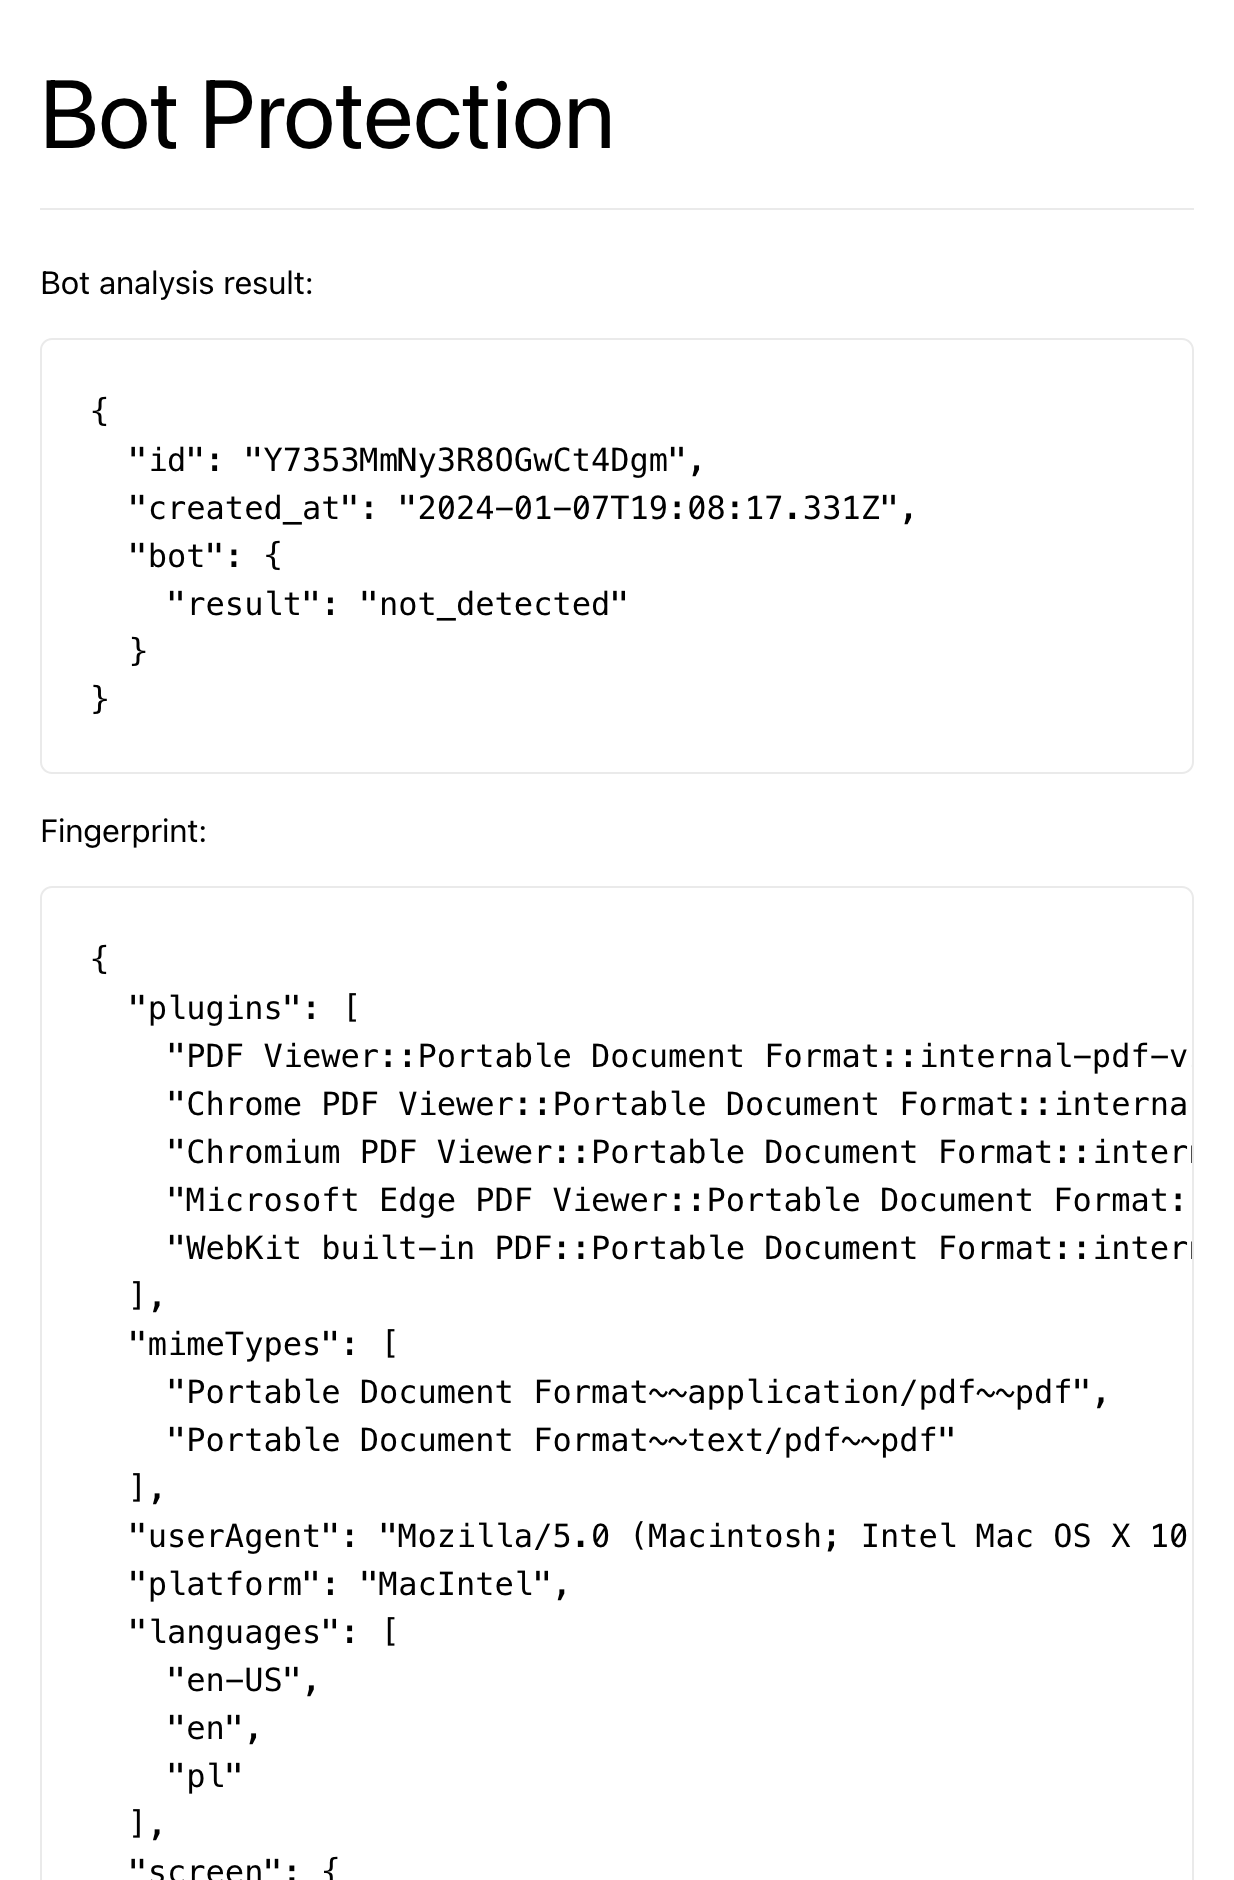
\includegraphics[width=0.5\textwidth]{img/bot-protection-not-detected}
        \caption{Wynik analizy odcisku standardowej przeglądarki}
        \label{fig:not-detected}
    \end{figure}
    \columnbreak
    \begin{figure}[H]
        \centering
        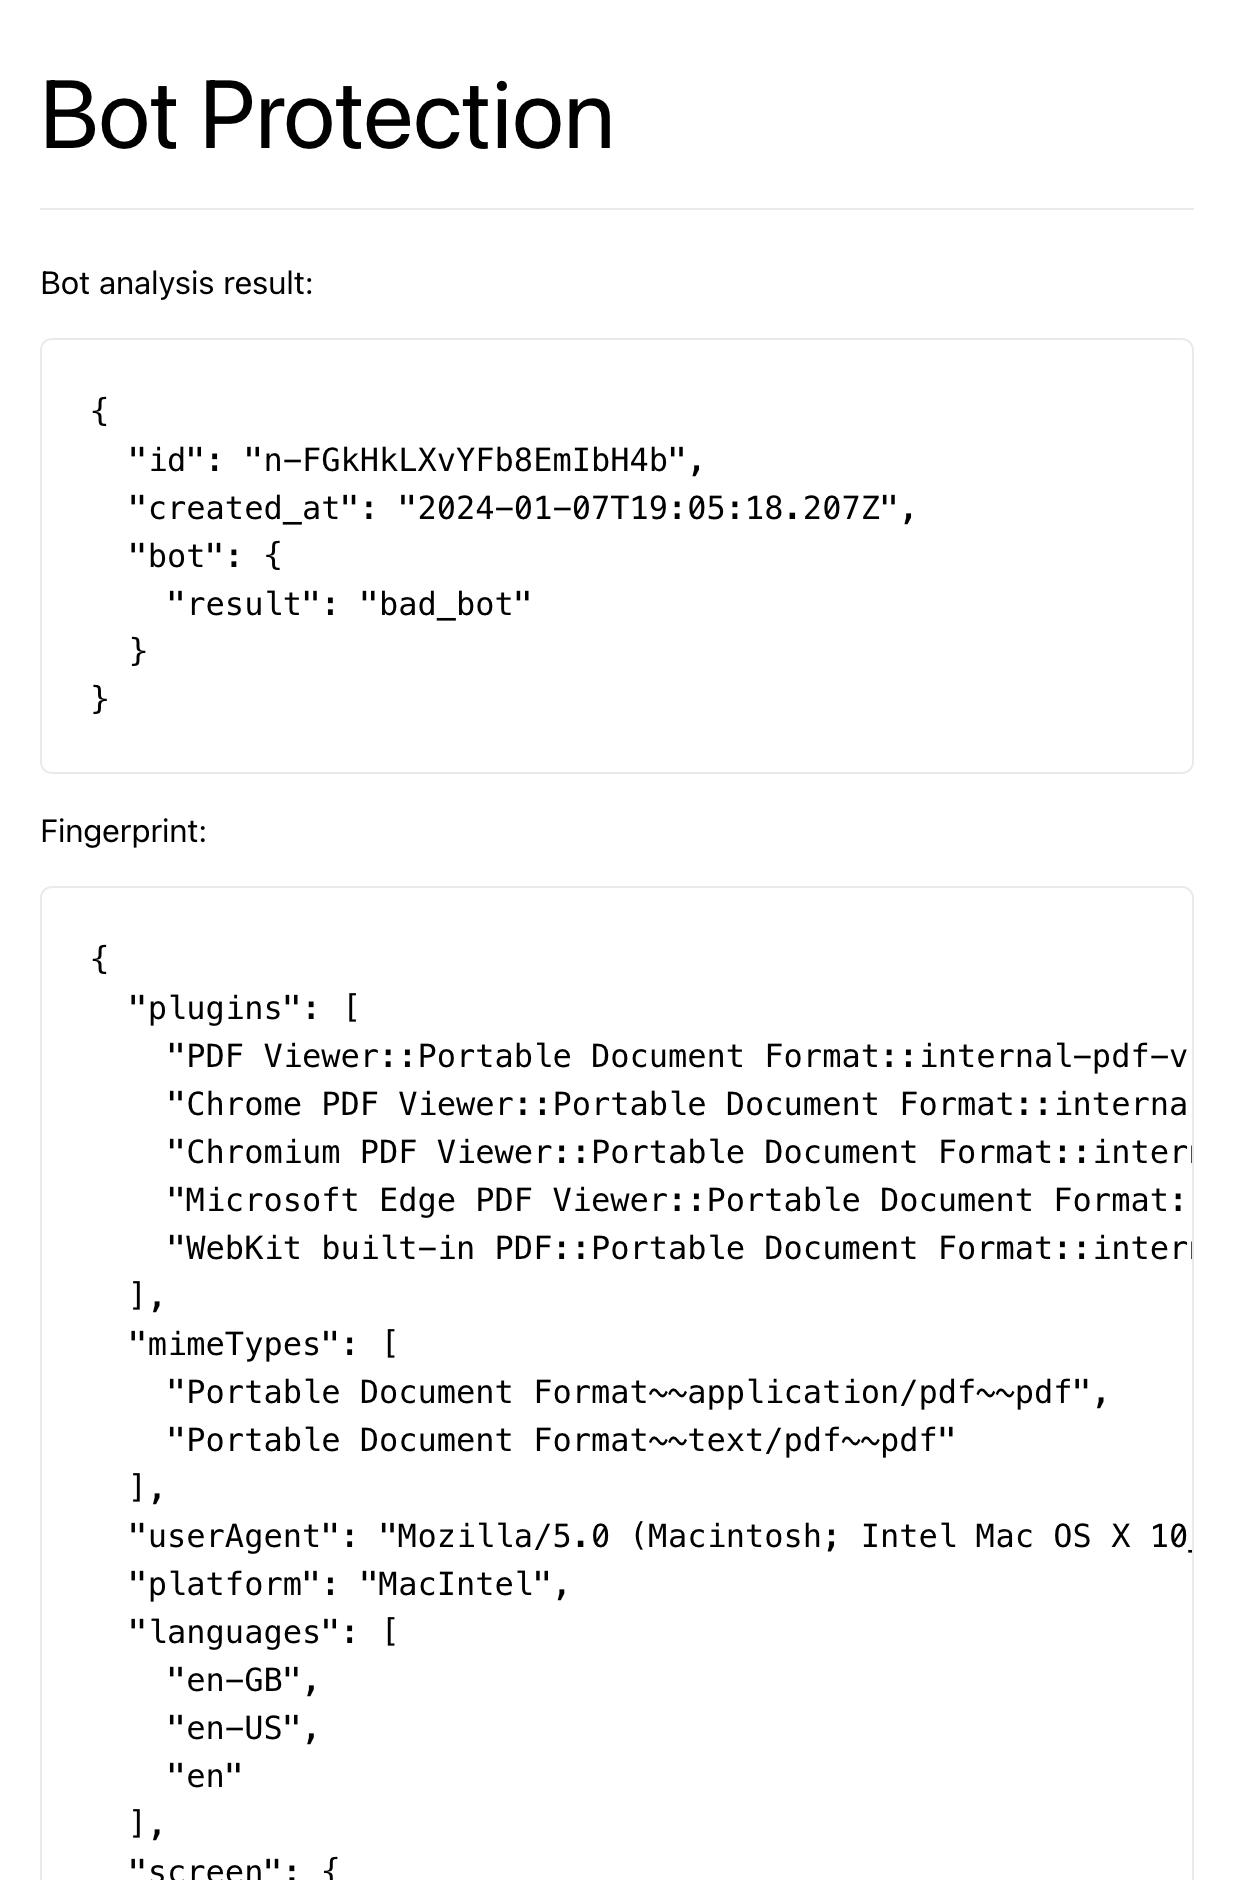
\includegraphics[width=0.5\textwidth]{img/bot-protection-bad-bot}
        \caption{Wynik analizy odcisku przeglądarki Chromium uruchomionej przez pupeteer}
        \label{fig:bad-bot-detected}
    \end{figure}
\end{multicols}

\subsection{Scenariusz 5: Włączone wszystkie zabezpieczenia}\label{subsec:scenariusz-5:-waczone-wszystkie-zapezpieczenia}

W piątym i ostatnim scenariuszu testowym, przetestowano działanie sklepu internetowego i scrapera przy jednoczesnym włączeniu wszystkich opisywanych zabezpieczeń tj. rate limiting, bot blocker reverse proxy oraz zabezpieczenia opartego na browser fingerprintingu.

Standardowi użytkownicy zachowali swobodny dostęp do sklepu internetowego tulski.
Komfort korzystania z serwisu pozostał bez zmian względem scenariusza 1.

Web scraper po uruchomieniu napotkał znaczne trudności w dostępie do zasobów sklepu internetowego.
Większość żądań została zablokowana przez rate limiting, a te które mieściły się w limicie zostały zablokowane przez mechanizm oparty o browser fingerprinting.
Próba pobrania danych całkowicie się nie powiodła.